\title{EE5311 -- Assignment 4}
\author{Joyen Benitto}
\date{\today}
\maketitle

\section{Problem 1: DRC and LVS clean CMOS reference inverter layout}

DRC and LVS clean layout of the CMOS reference inverter
($W_p/L_p = 0.84/0.15\ \mu\text{m}$, $W_n/L_n = 0.42/0.15\ \mu\text{m}$).
The extracted netlist (\texttt{inv\_extracted.cir}) is used for both inverter
instances in the delay testbench below.

\subsection*{Schematic}
The below is the two-inverter delay testbench (\texttt{inv\_tb.sch} /
\texttt{assign1a.sch}), with net \texttt{vout1} tapped between the driving
and load inverter instances. The testbench includes the extracted netlist
(\texttt{inv\_tb\_extracted.spice}), applies a PULSE input, and measures the
rise/fall delay to \texttt{v(out1)}.

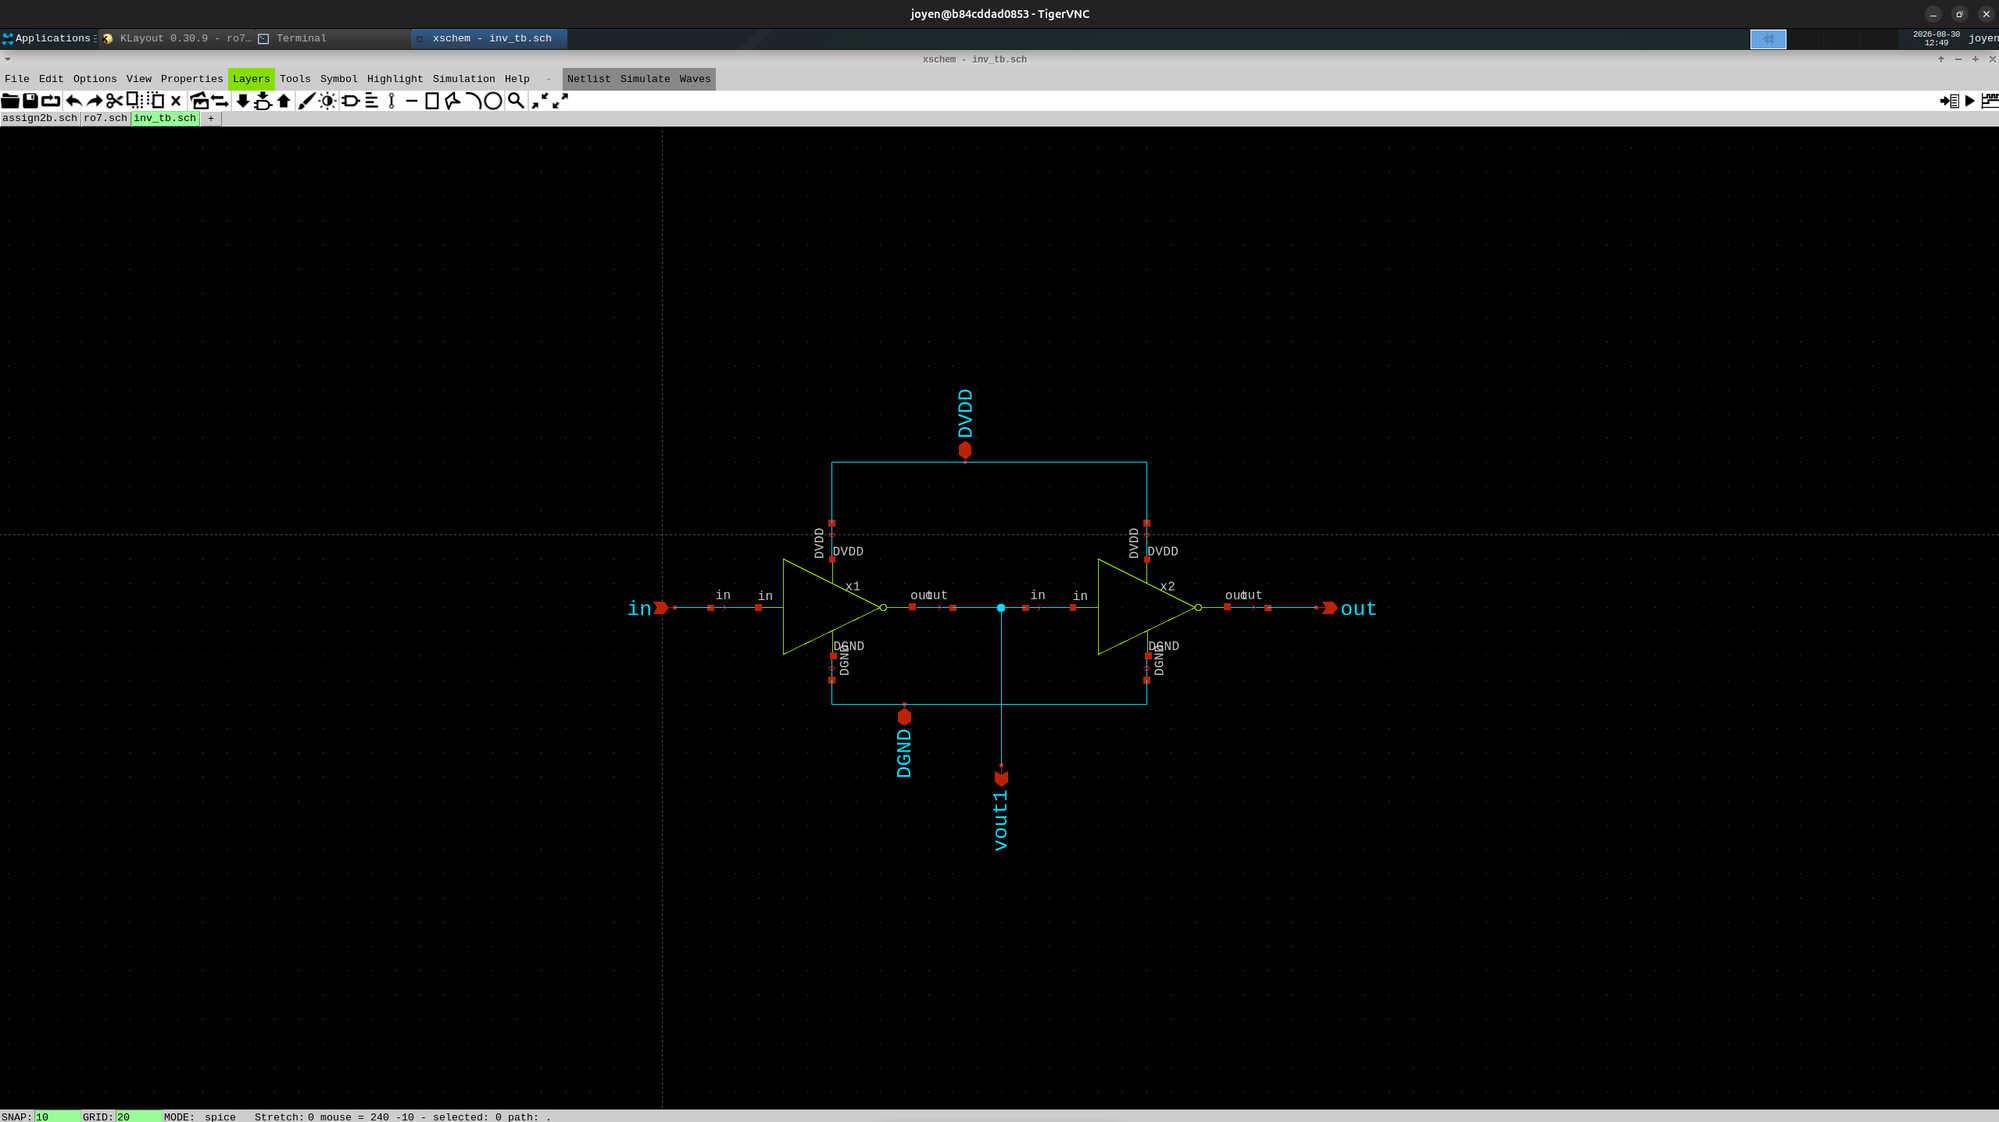
\includegraphics[width=0.9\textwidth]{figures/inv_tb_schematic_1a.png}

\textbf{Figure 1:} \texttt{assign1a.sch} -- two extracted inverter instances, net \texttt{vout1} tapped

This schematic is common to both parts below; only the netlist used for the
delay measurement differs.

%%------------------------------------------------------------------------------
\subsection{Extract the parasitic values from the layout and find the delay of the inverter}

\subsubsection{Layout}
The below is the standalone DRC/LVS-clean inverter layout (\texttt{inv.gds})
that gets parasitic-extracted to \texttt{inv\_extracted.cir}; this extracted
netlist is instantiated for both inverter instances in the testbench.

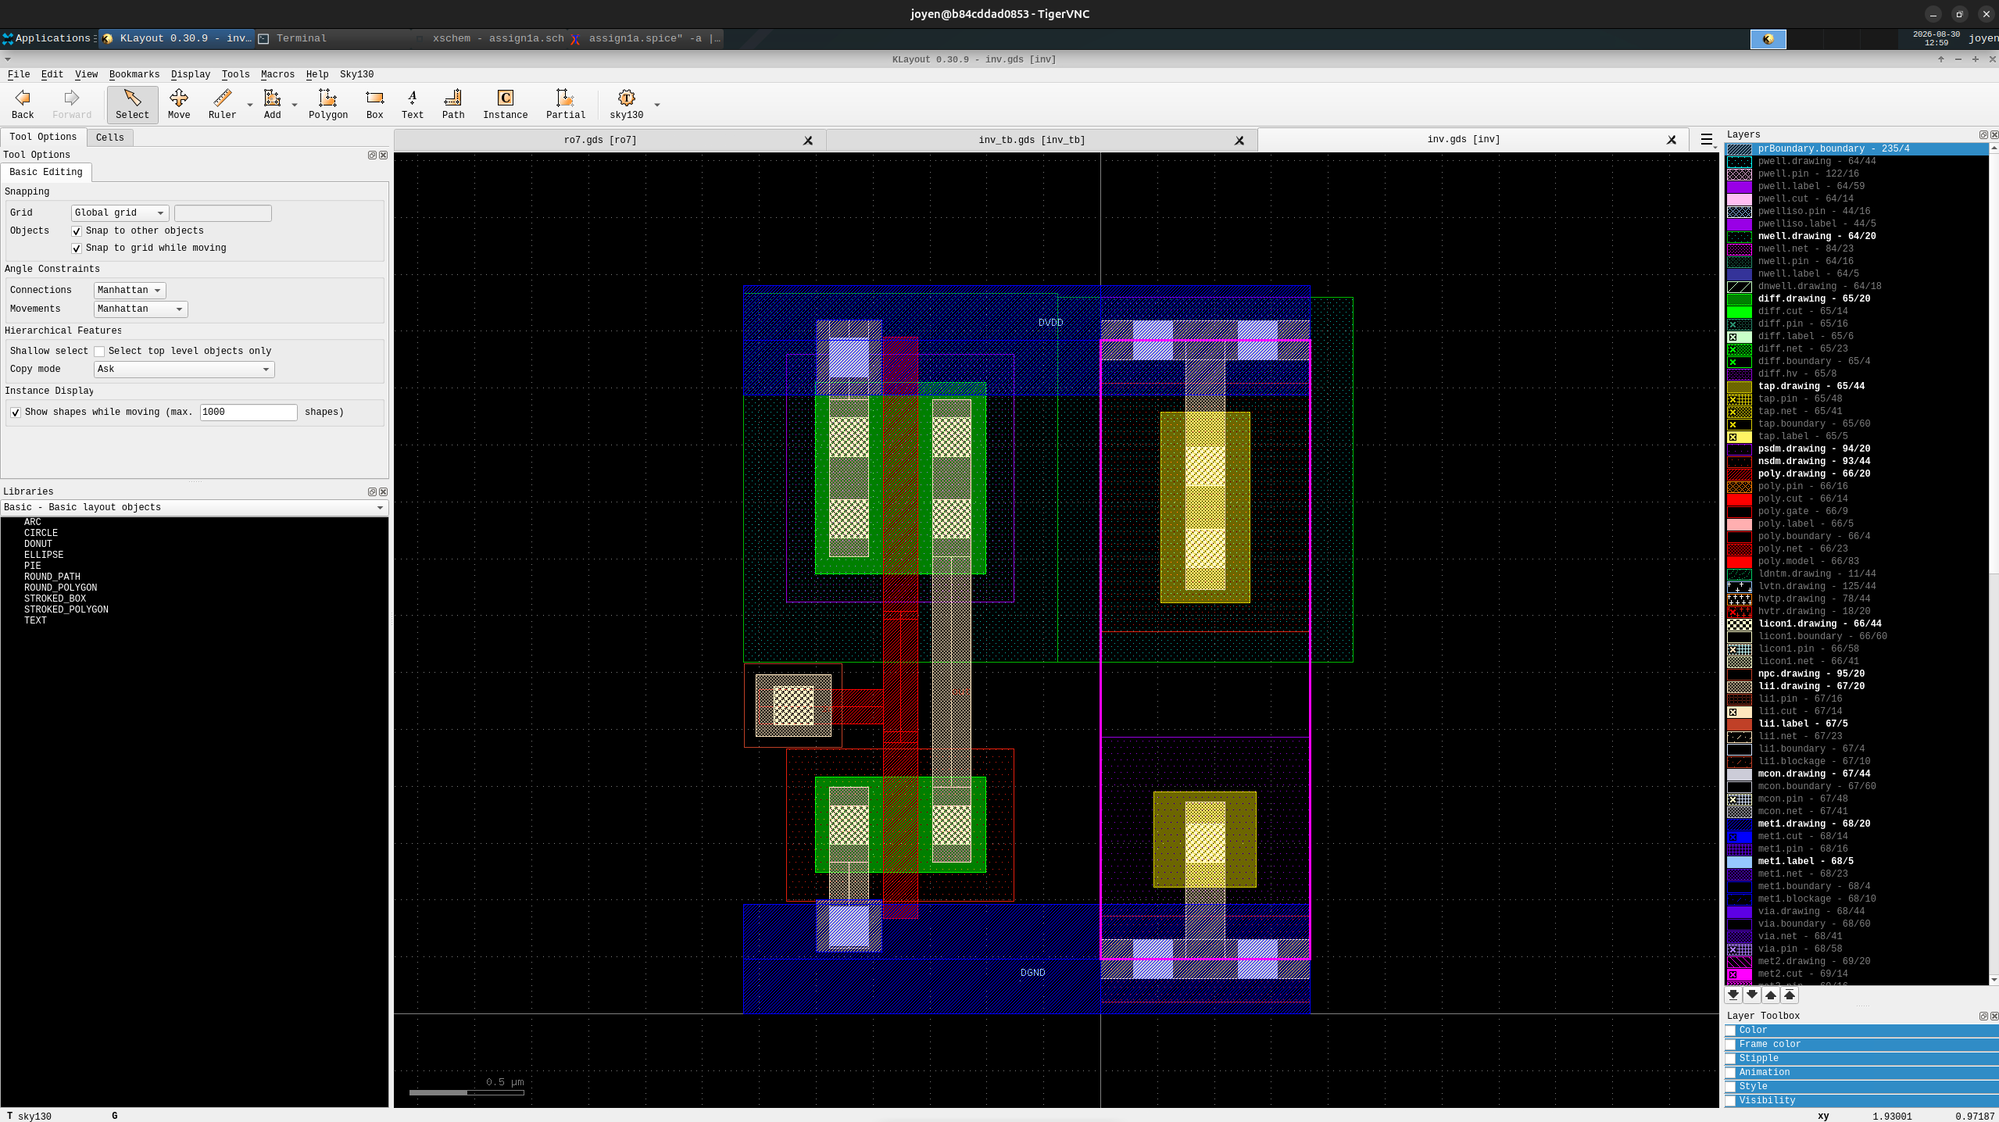
\includegraphics[width=0.9\textwidth]{figures/inv_gds_1a.png}

\textbf{Figure 2:} \texttt{inv.gds} (KLayout) -- standalone reference inverter layout

\subsubsection{Measurement}

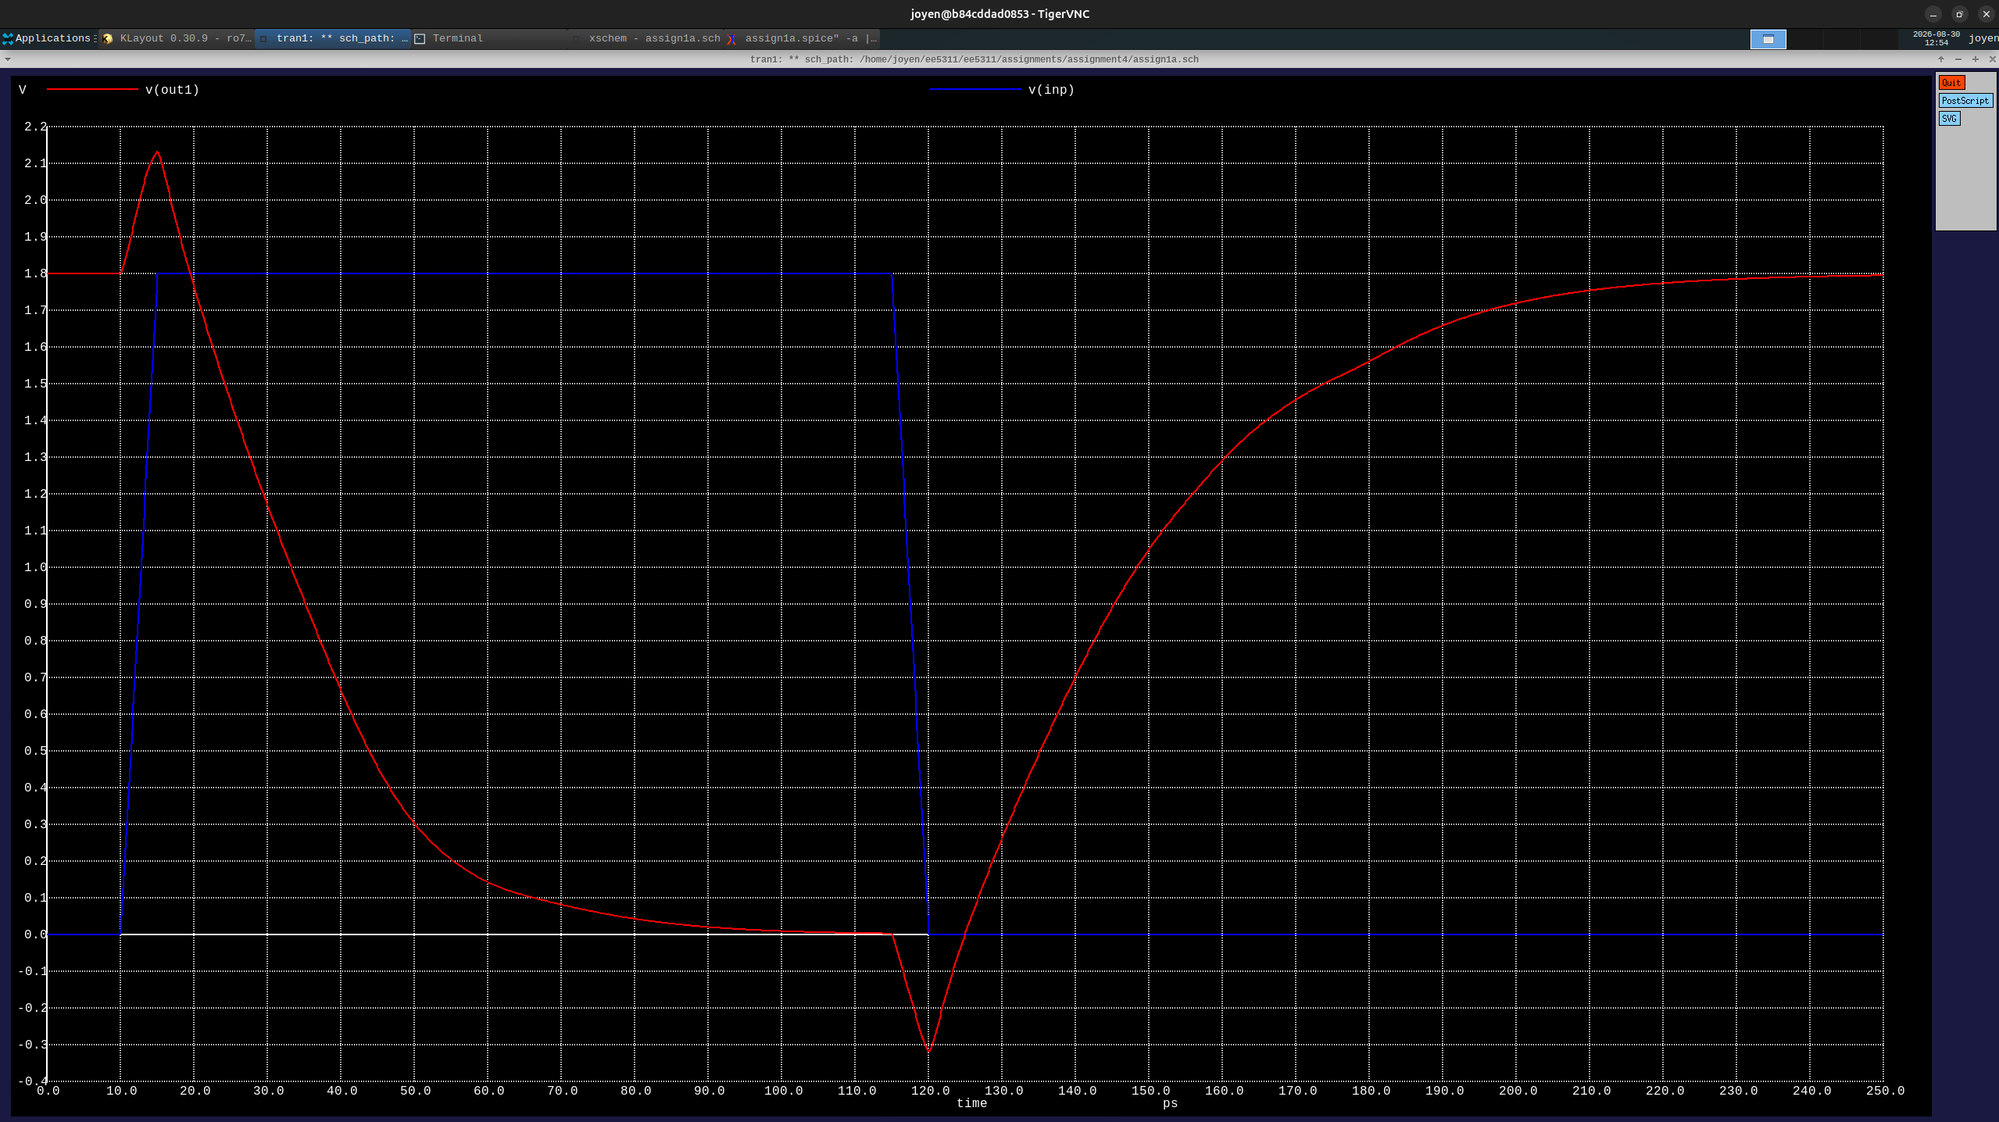
\includegraphics[width=0.9\textwidth]{figures/inv_tb_delay_tran_1a.jpeg}

\textbf{Figure 3:} $v(out1)$ vs $v(inp)$, extracted netlist, 250~ps transient

\[
\begin{aligned}
t_{pLH} &= 1.452402 \times 10^{-10} - 1.250000 \times 10^{-11} = 1.327402 \times 10^{-10}\ \text{s} \\
t_{pHL} &= 3.517798 \times 10^{-11} - 1.175000 \times 10^{-10} = -8.232202 \times 10^{-11}\ \text{s} \\
t_p &= \frac{t_{pLH} + t_{pHL}}{2} = 2.5209 \times 10^{-11}\ \text{s} = 25.209\ \text{ps}
\end{aligned}
\]

The propagation delay of the inverter, using the extracted netlist for both
instances, is $\approx 25.2$~ps.
%%------------------------------------------------------------------------------
\subsection{Measure the delay including the layout parasitics of net Vout}

\subsubsection{Layout}
The below is the two-inverter testbench layout (\texttt{inv\_tb.gds}): two
instances of the reference inverter (\texttt{inv.gds}) placed back to back,
with net \texttt{vout1} (the net whose layout parasitics are extracted here)
running between the driving inverter's output and the load inverter's input.

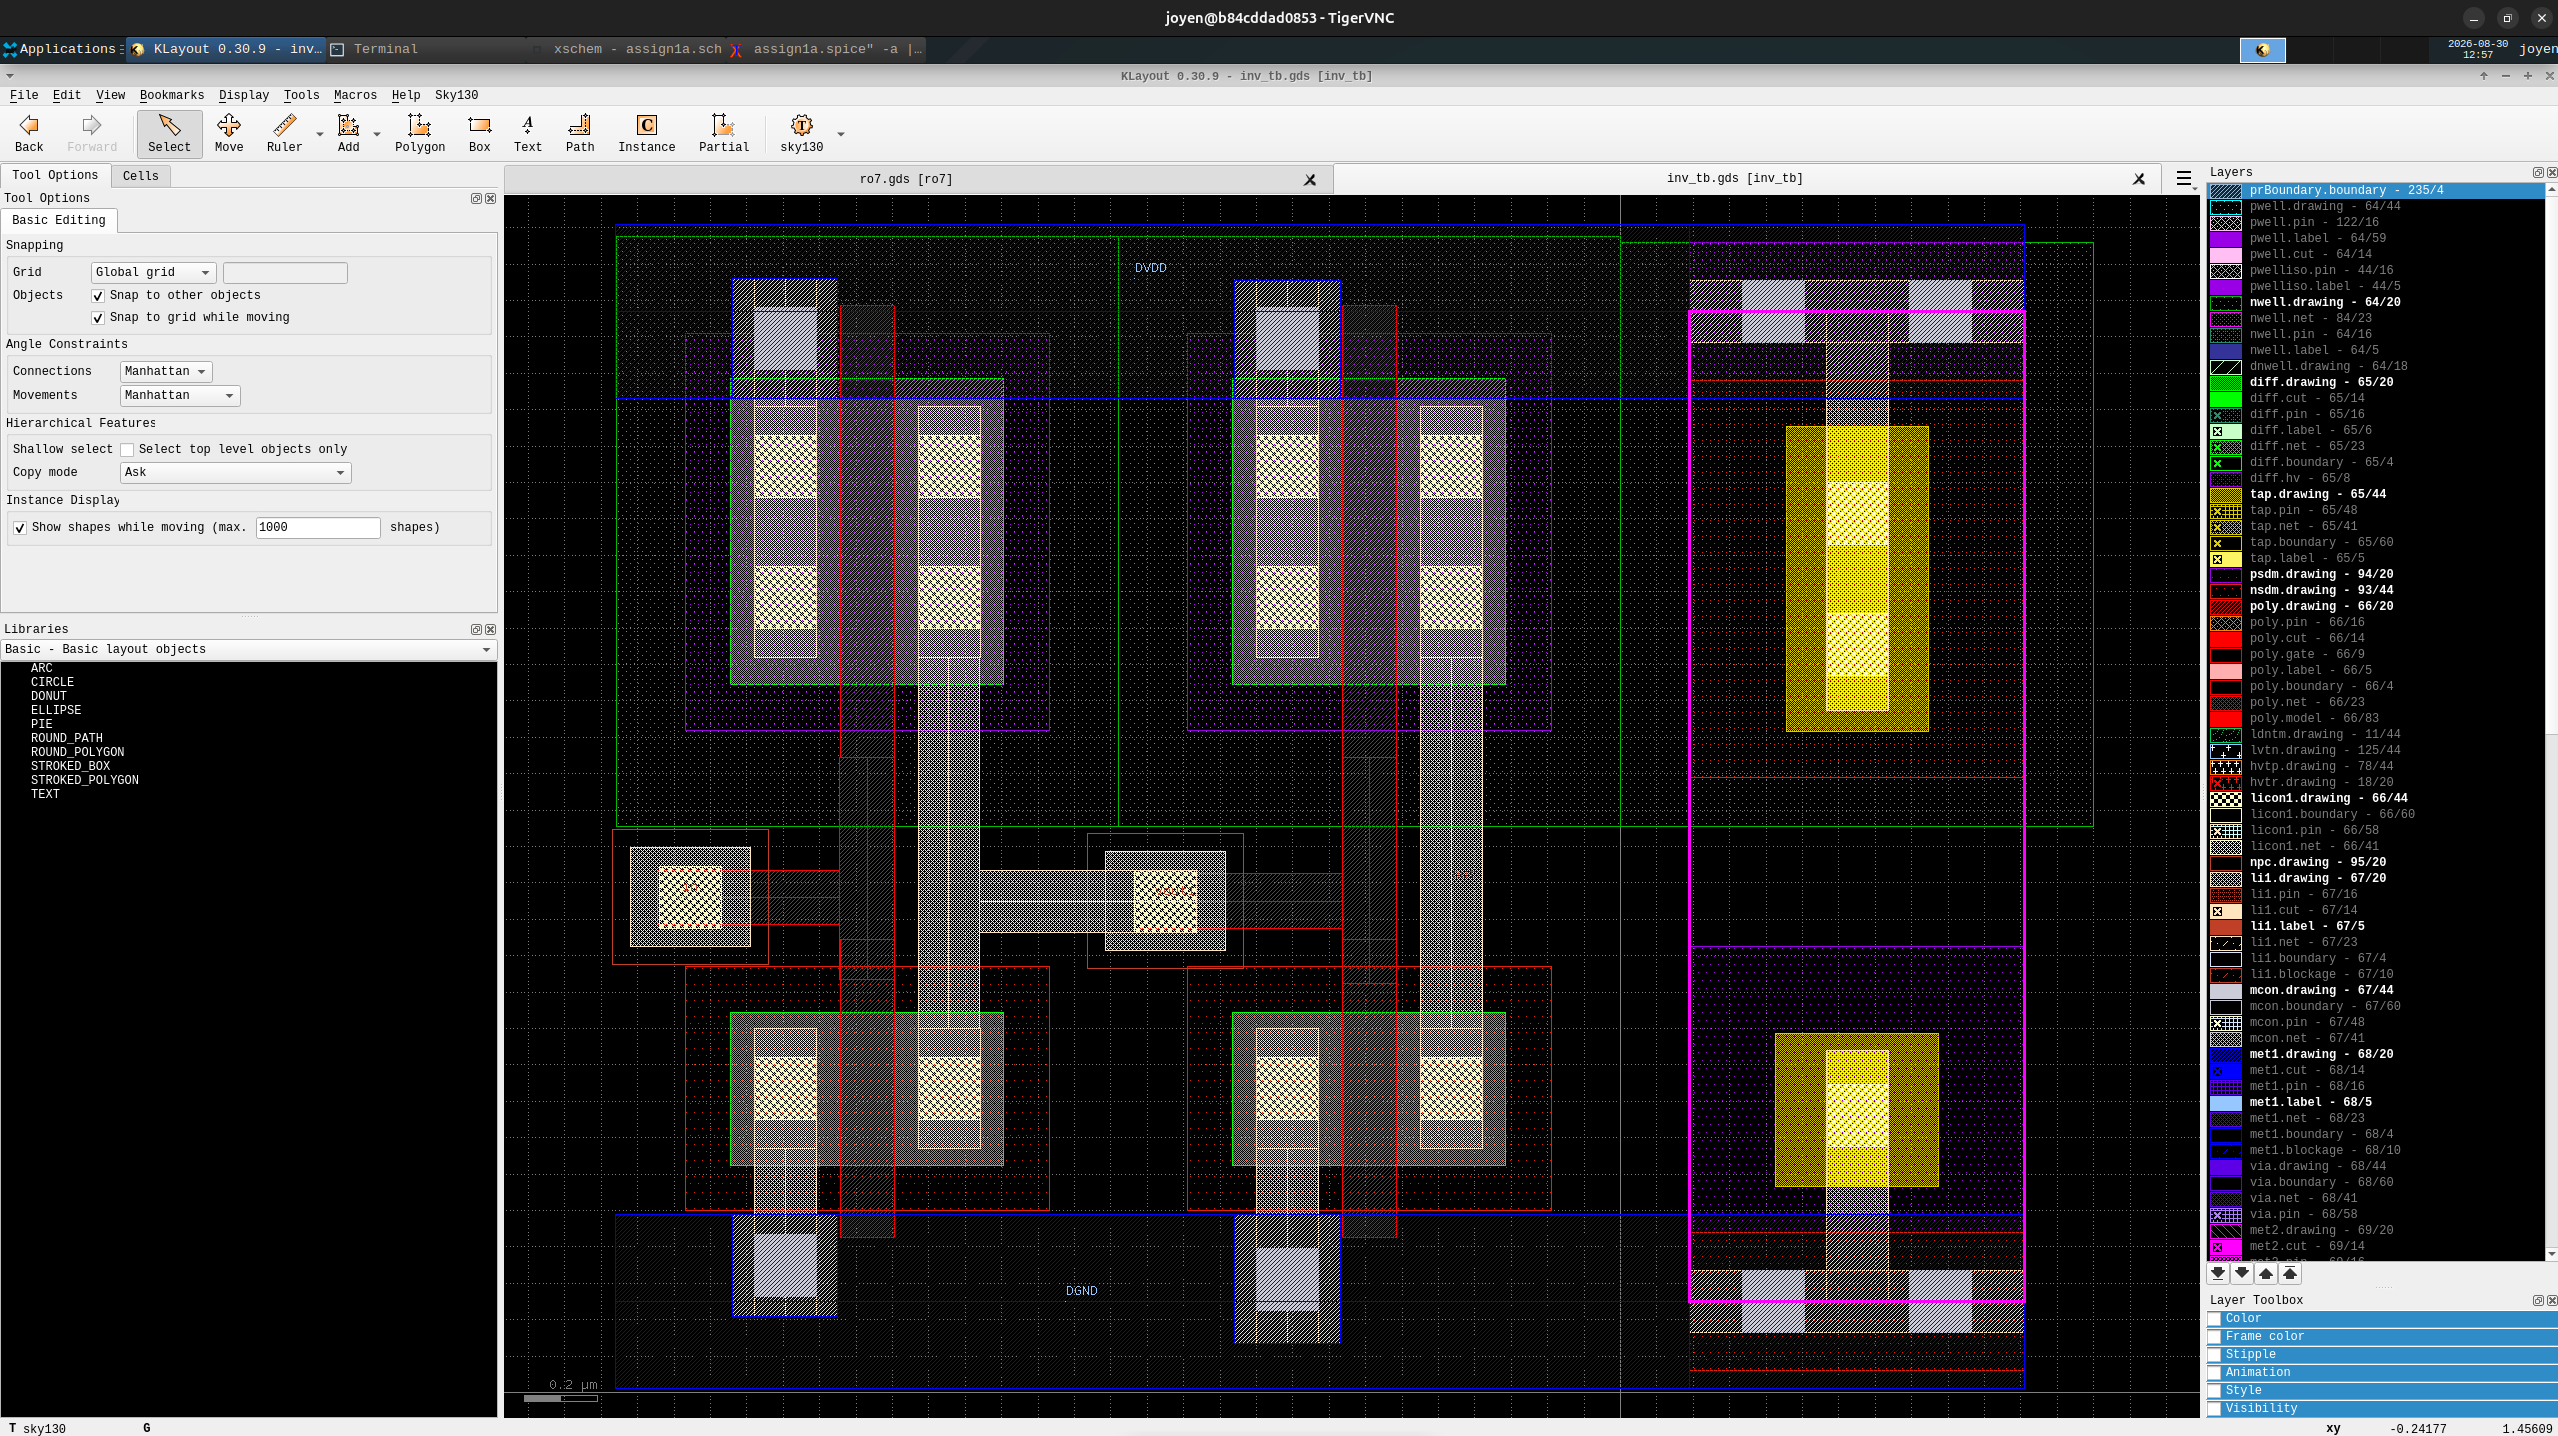
\includegraphics[width=0.9\textwidth]{figures/inv_gds_1b.png}

\textbf{Figure 4:} \texttt{inv\_tb.gds} (KLayout) -- two inverter instances, net \texttt{vout1} tapped between them

\subsubsection{Measurement}
Same extracted-netlist simulation as Section~1.1: the delay of net
\texttt{vout1} (which already carries the layout-extracted parasitic R/C from
\texttt{inv\_tb\_extracted.spice}) is $\approx 25.2$~ps -- see
Section~1.1 for the waveform and \texttt{tlh}/\texttt{thl} calculation.
%%------------------------------------------------------------------------------
\section{Problem 2: Ring oscillator}

\subsection{Measure the oscillating frequency for VDD = 1.8V with the layout parasitics.}

\subsubsection{Schematic}
The below is a xschem schematic for the ring oscillator

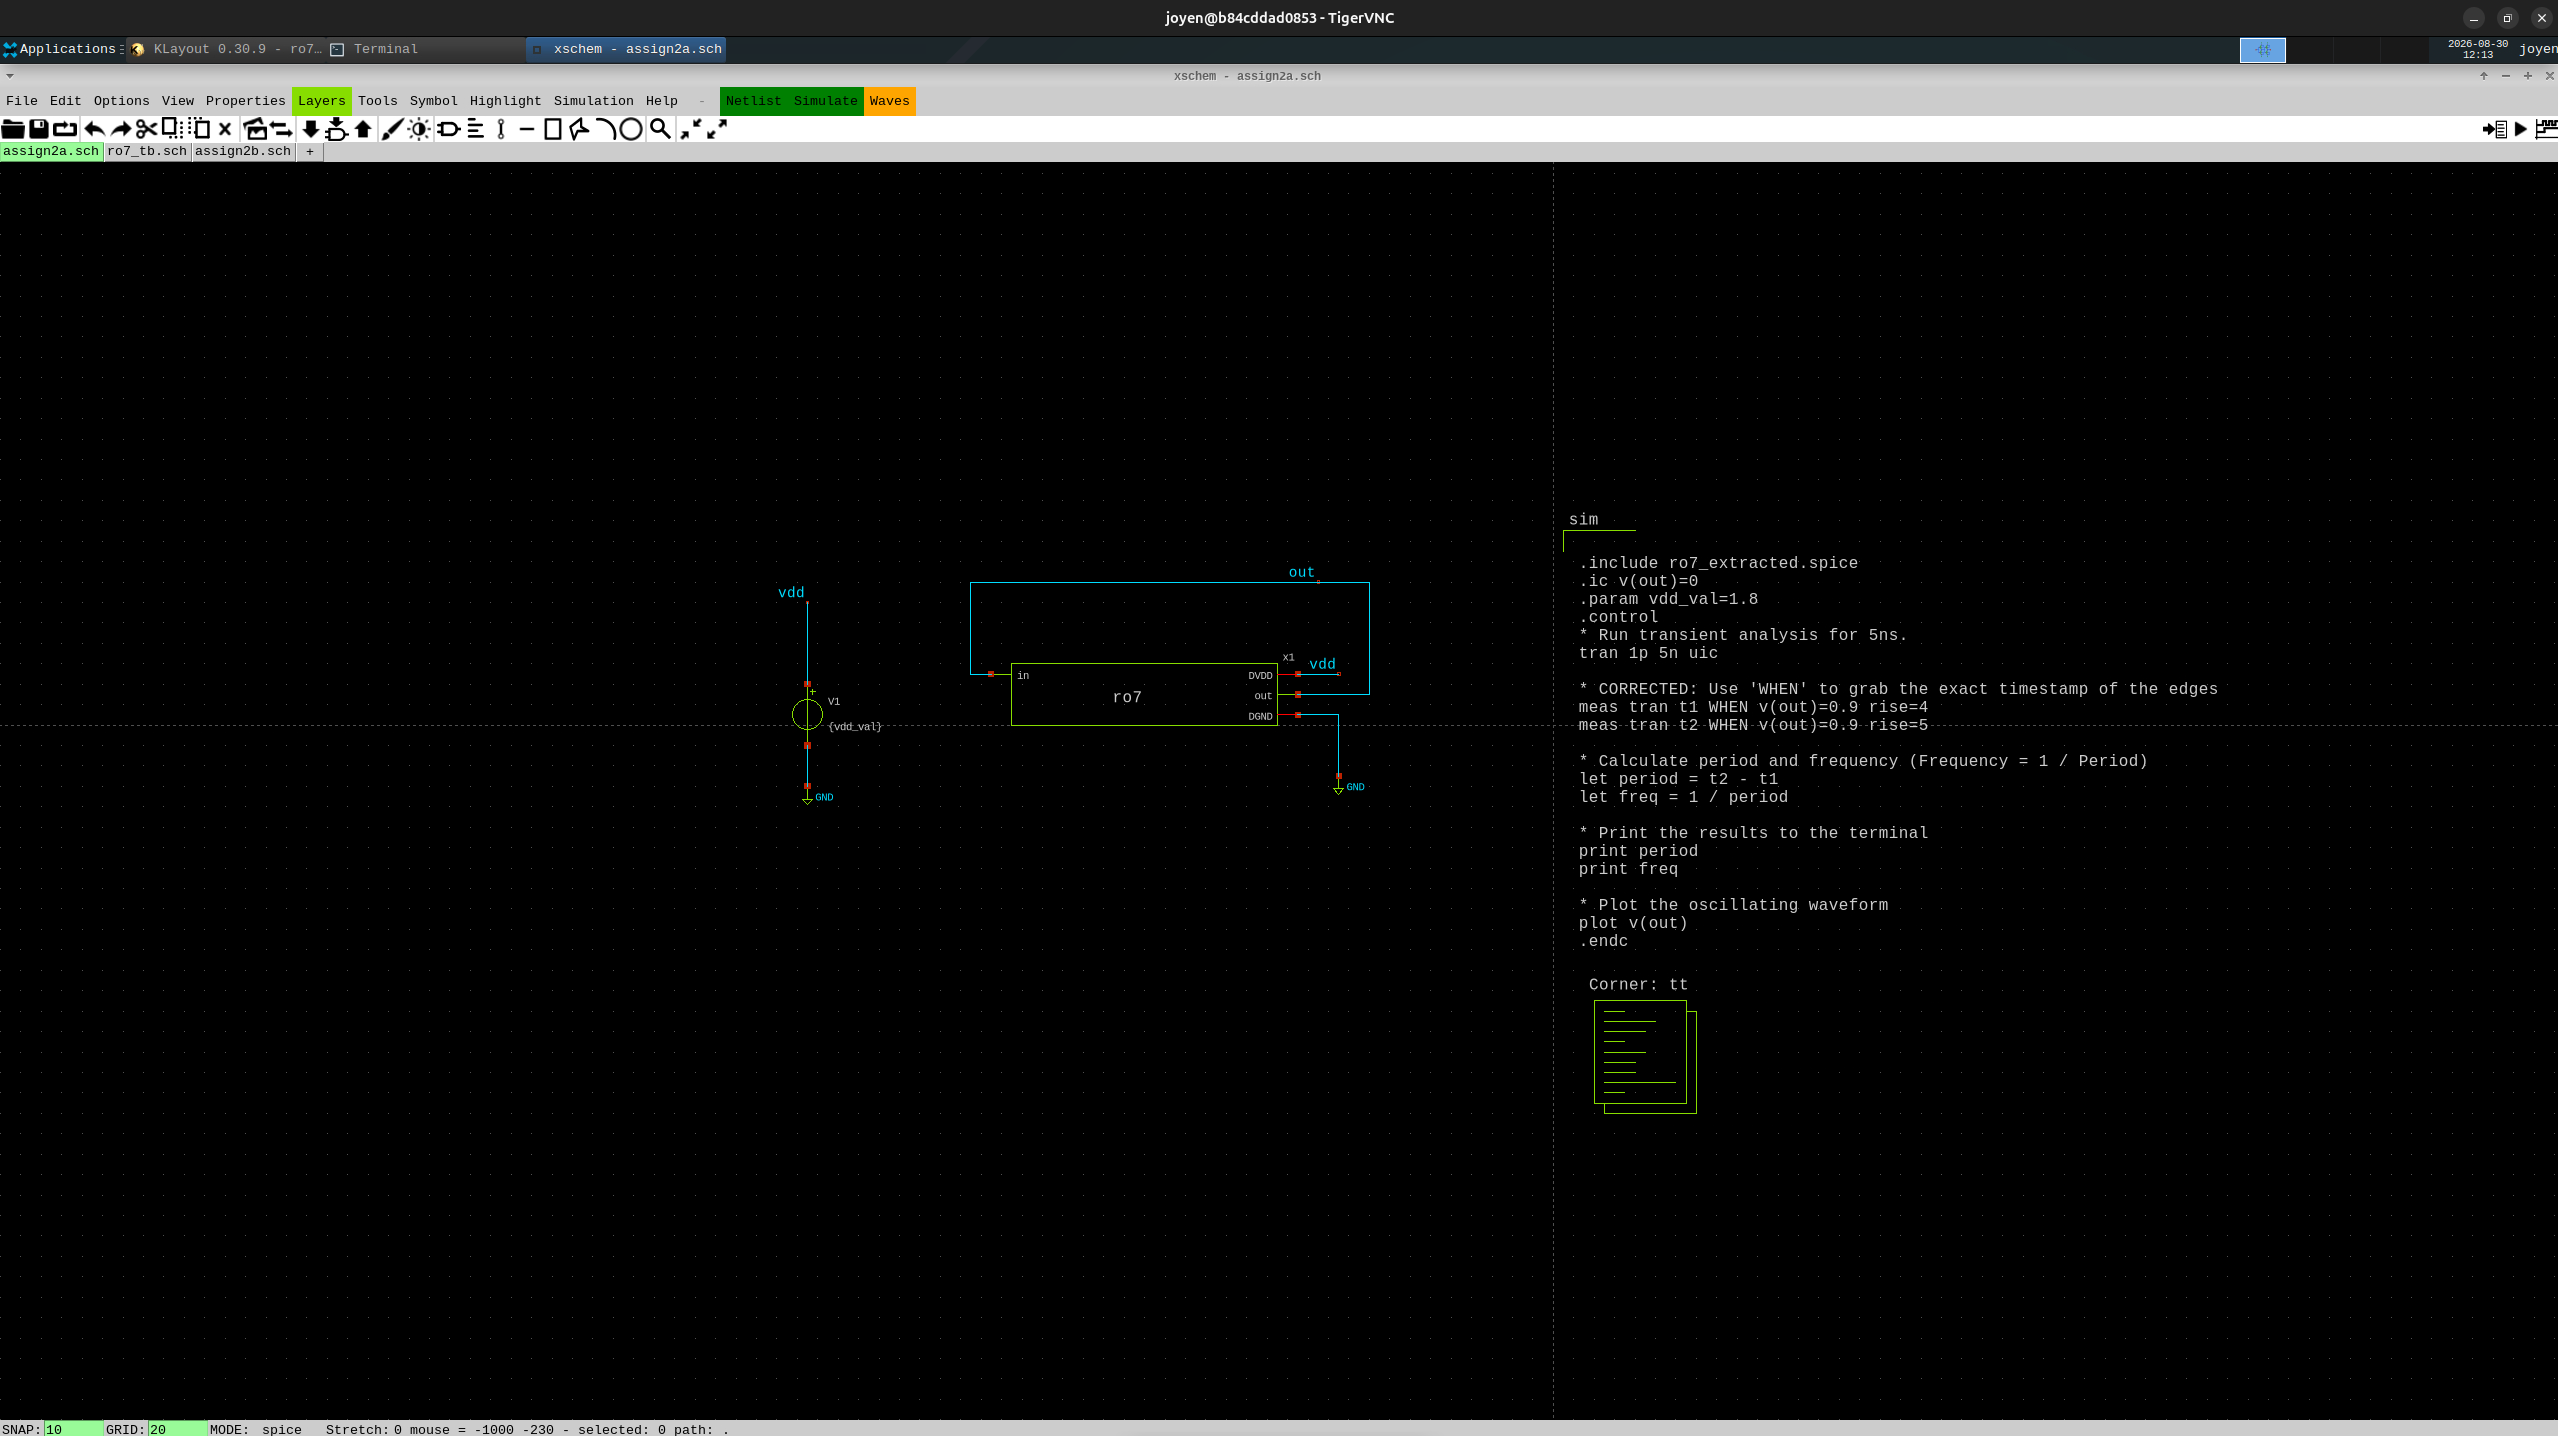
\includegraphics[width=0.9\textwidth]{figures/ro7_schematic_2a.png}

\textbf{Figure 5:} xschem schematic

\subsubsection{Layout}

The below is the layout of the ring oscillator

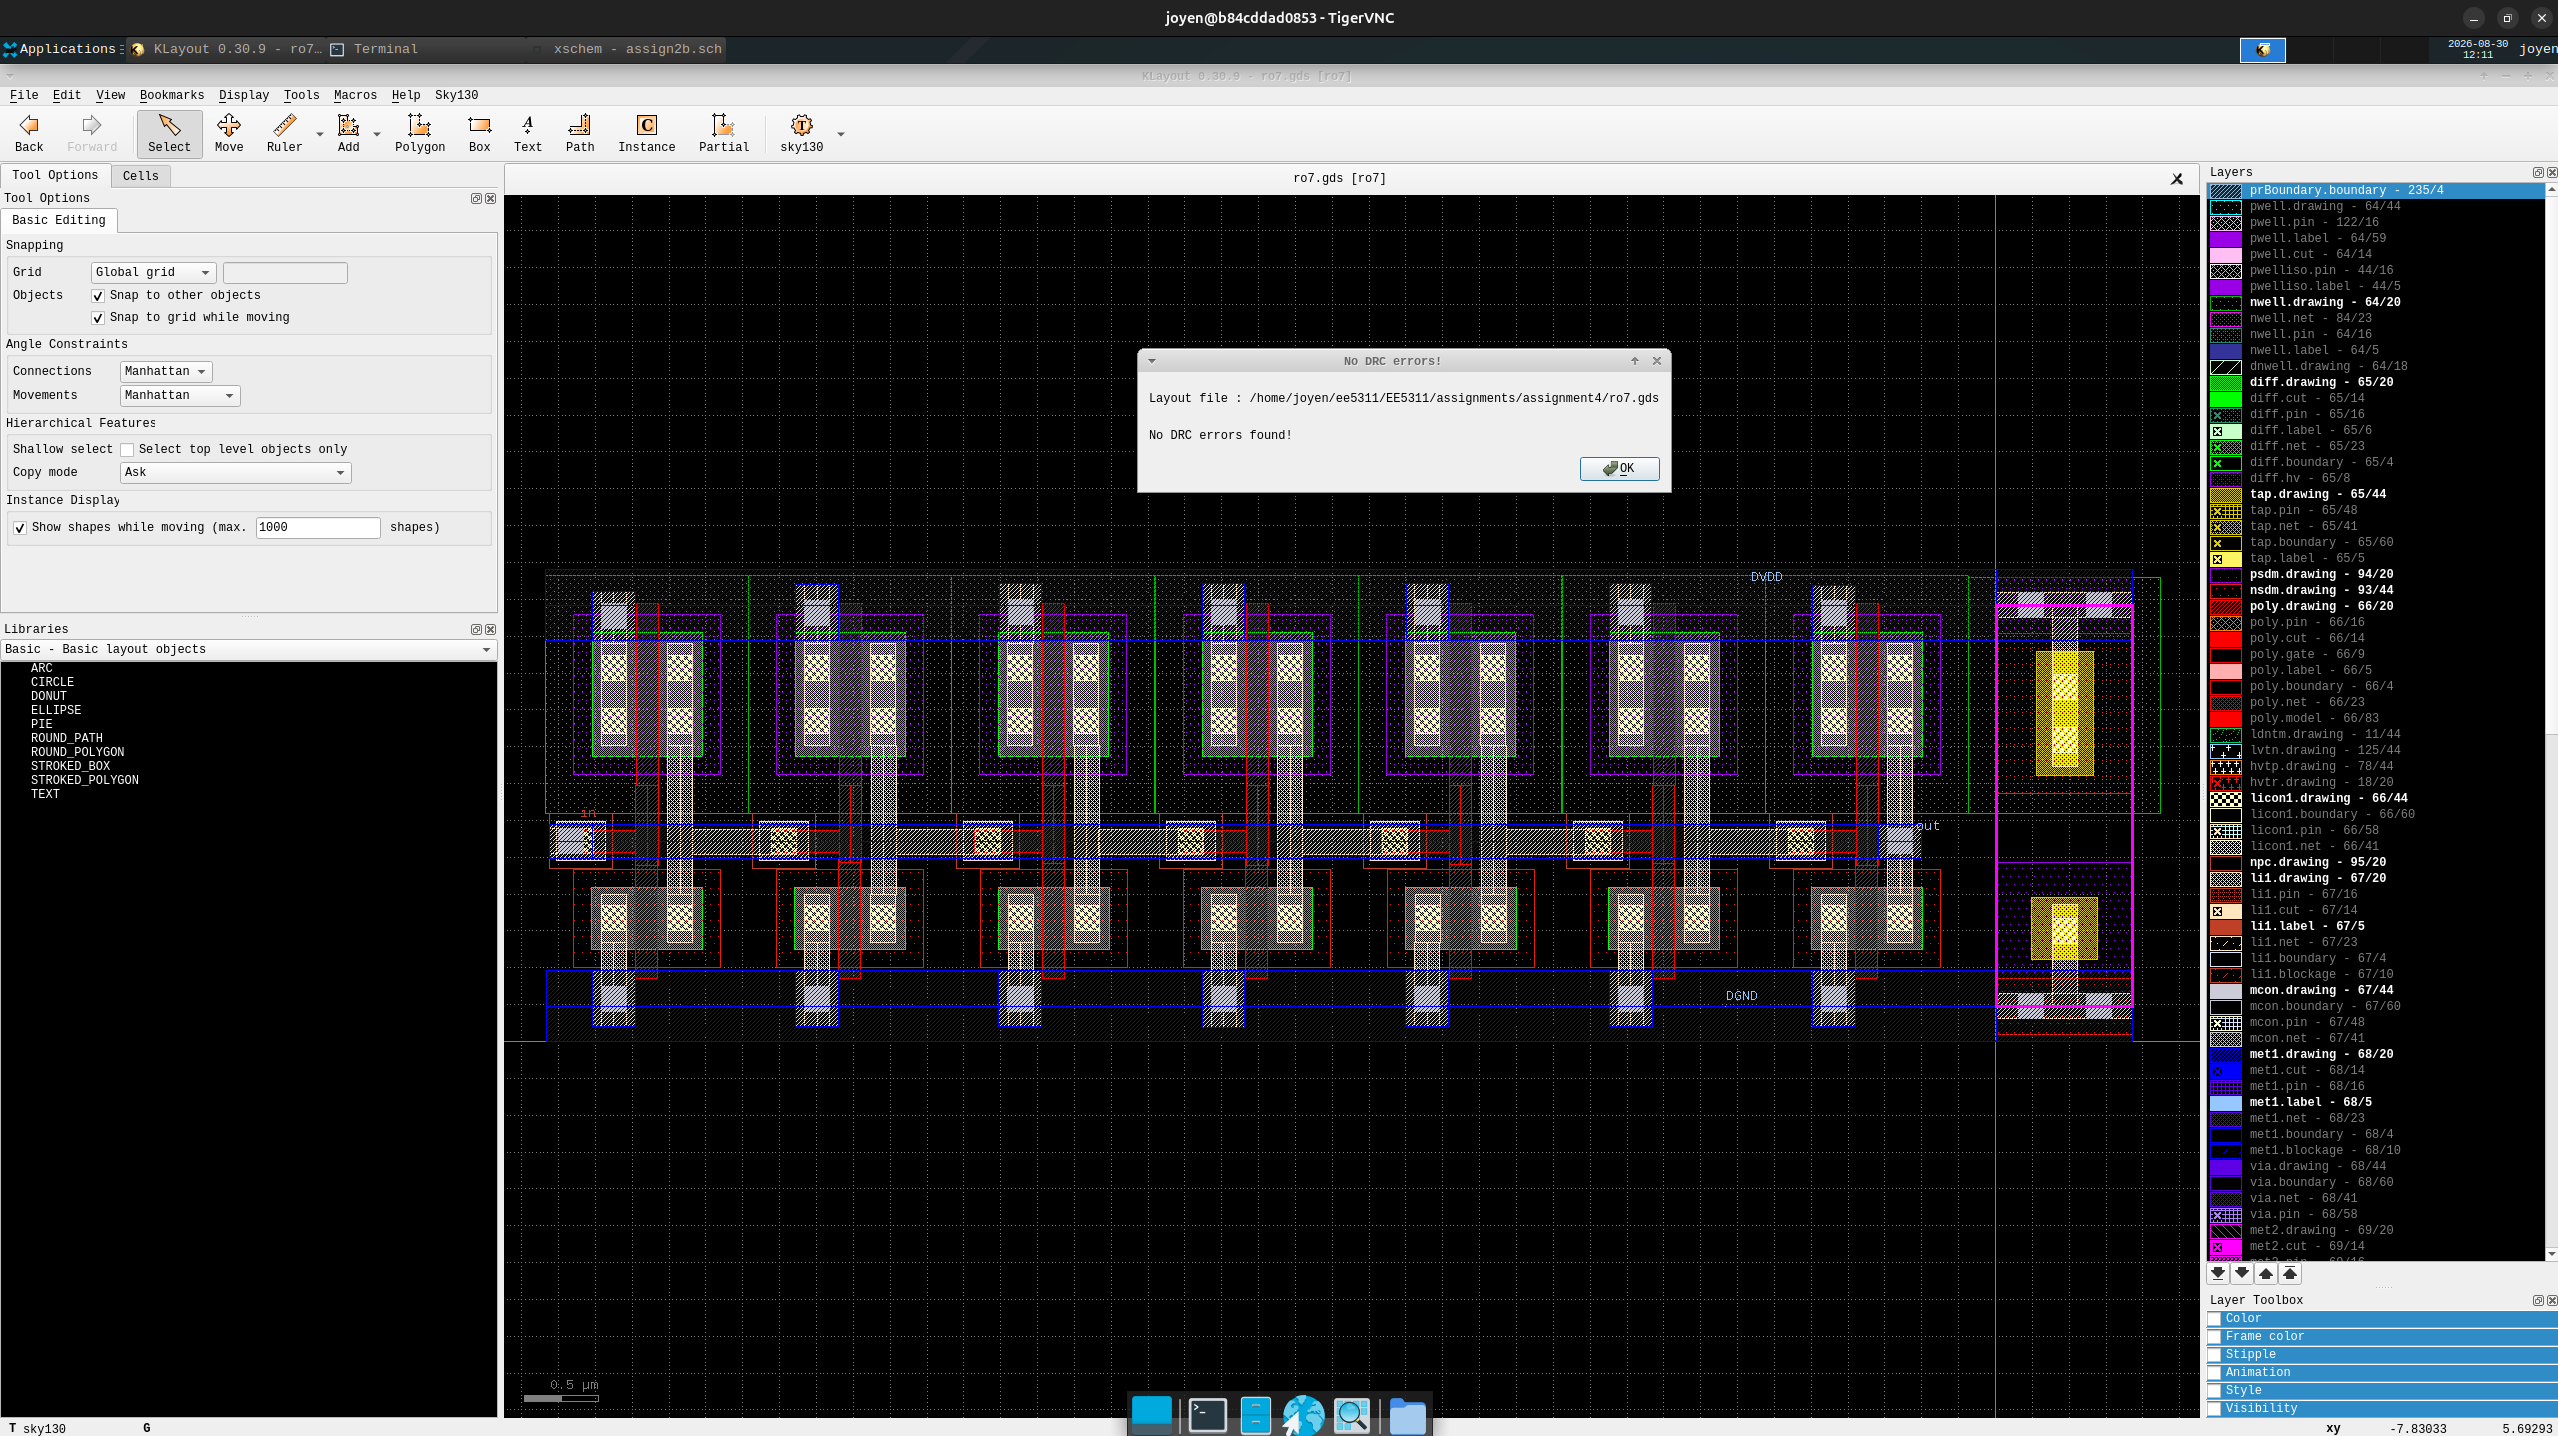
\includegraphics[width=0.9\textwidth]{figures/ro7_layout.png}

\textbf{Figure 6:} ring oscillator layout

\subsubsection{Measurement}

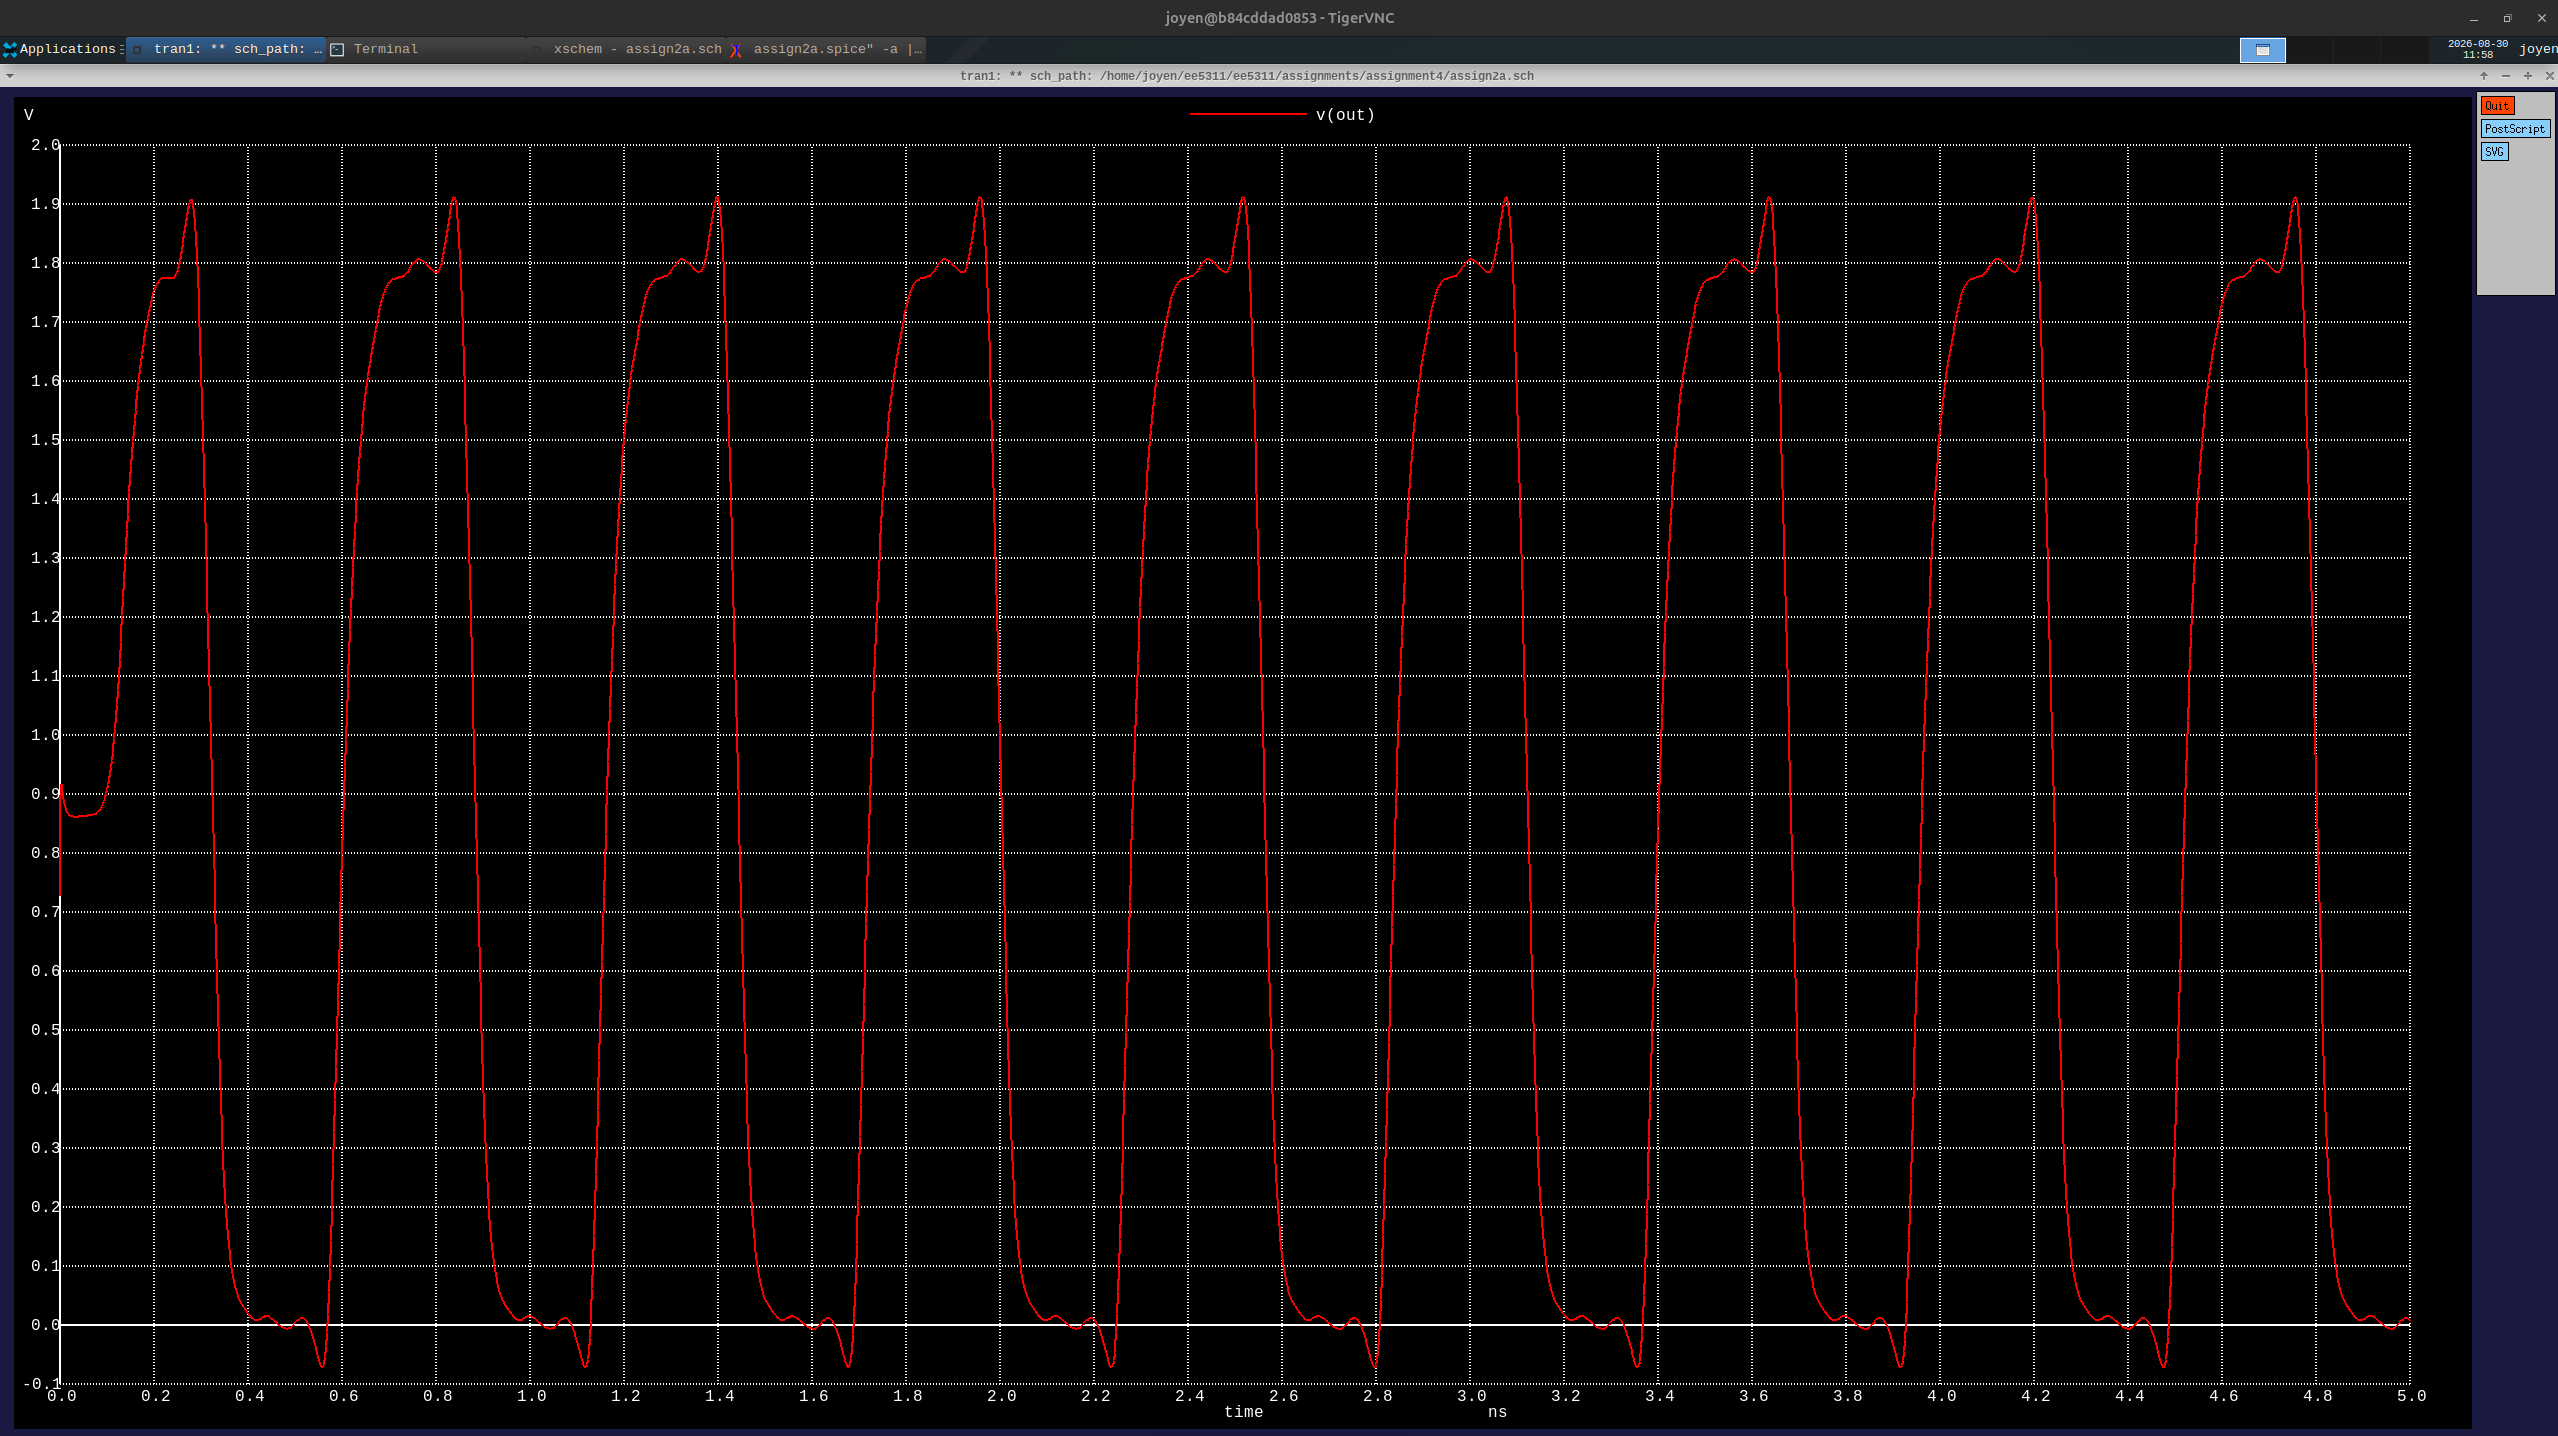
\includegraphics[width=0.9\textwidth]{figures/ro7_oscillating_2a.png}

\textbf{Figure 7:} $V_{out}$ vs Time

\[
\begin{aligned}
t_1 &= 1.163440 \times 10^{-9}\ \text{s} \\
t_2 &= 1.723090 \times 10^{-9}\ \text{s} \\
\text{period} &= 5.596500 \times 10^{-10}\ \text{s} \\
\text{freq} &= 1.786831 \times 10^{9}\ \text{Hz}
\end{aligned}
\]

%%------------------------------------------------------------------------------
\subsection{Plot the oscillating frequency and time period as a function of VDD for VDD = 1V to 1.8V in steps
of 0.1V}
\subsubsection{Schematic}
The below testbench sweeps $V_{DD}$ from 1.0V to 1.8V in 0.1V steps using
\texttt{alterparam} in a \texttt{while} loop, measuring the period and
frequency at each step.

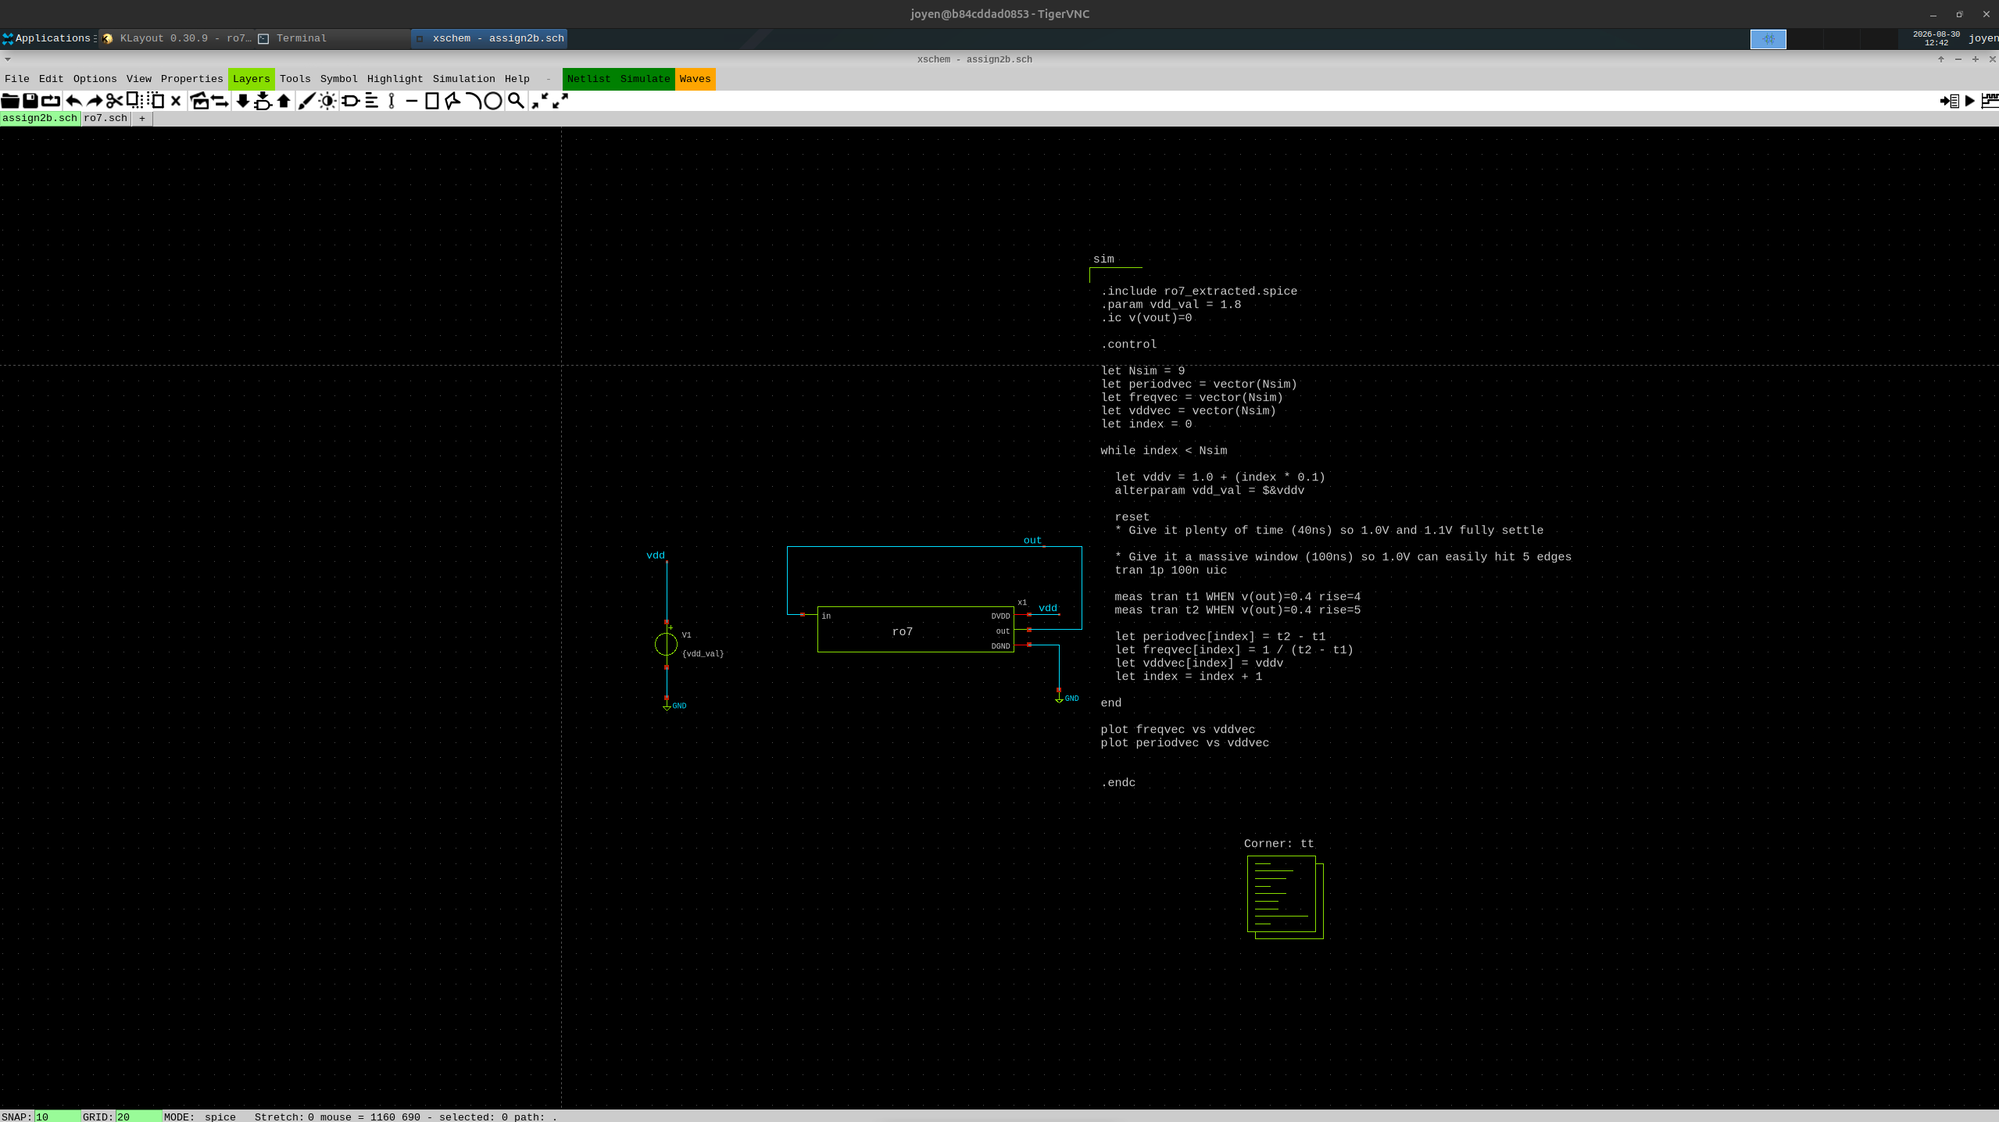
\includegraphics[width=0.9\textwidth]{figures/ro7_schematic_2b.png}

\textbf{Figure 8:} xschem schematic (\texttt{assign2b.sch}) with the $V_{DD}$ sweep script

\subsubsection{Layout}
Same ring oscillator layout as Section~2.1.2 (\texttt{ro7.gds}); only the
supply voltage is swept in simulation.

\subsubsection{Measurement}

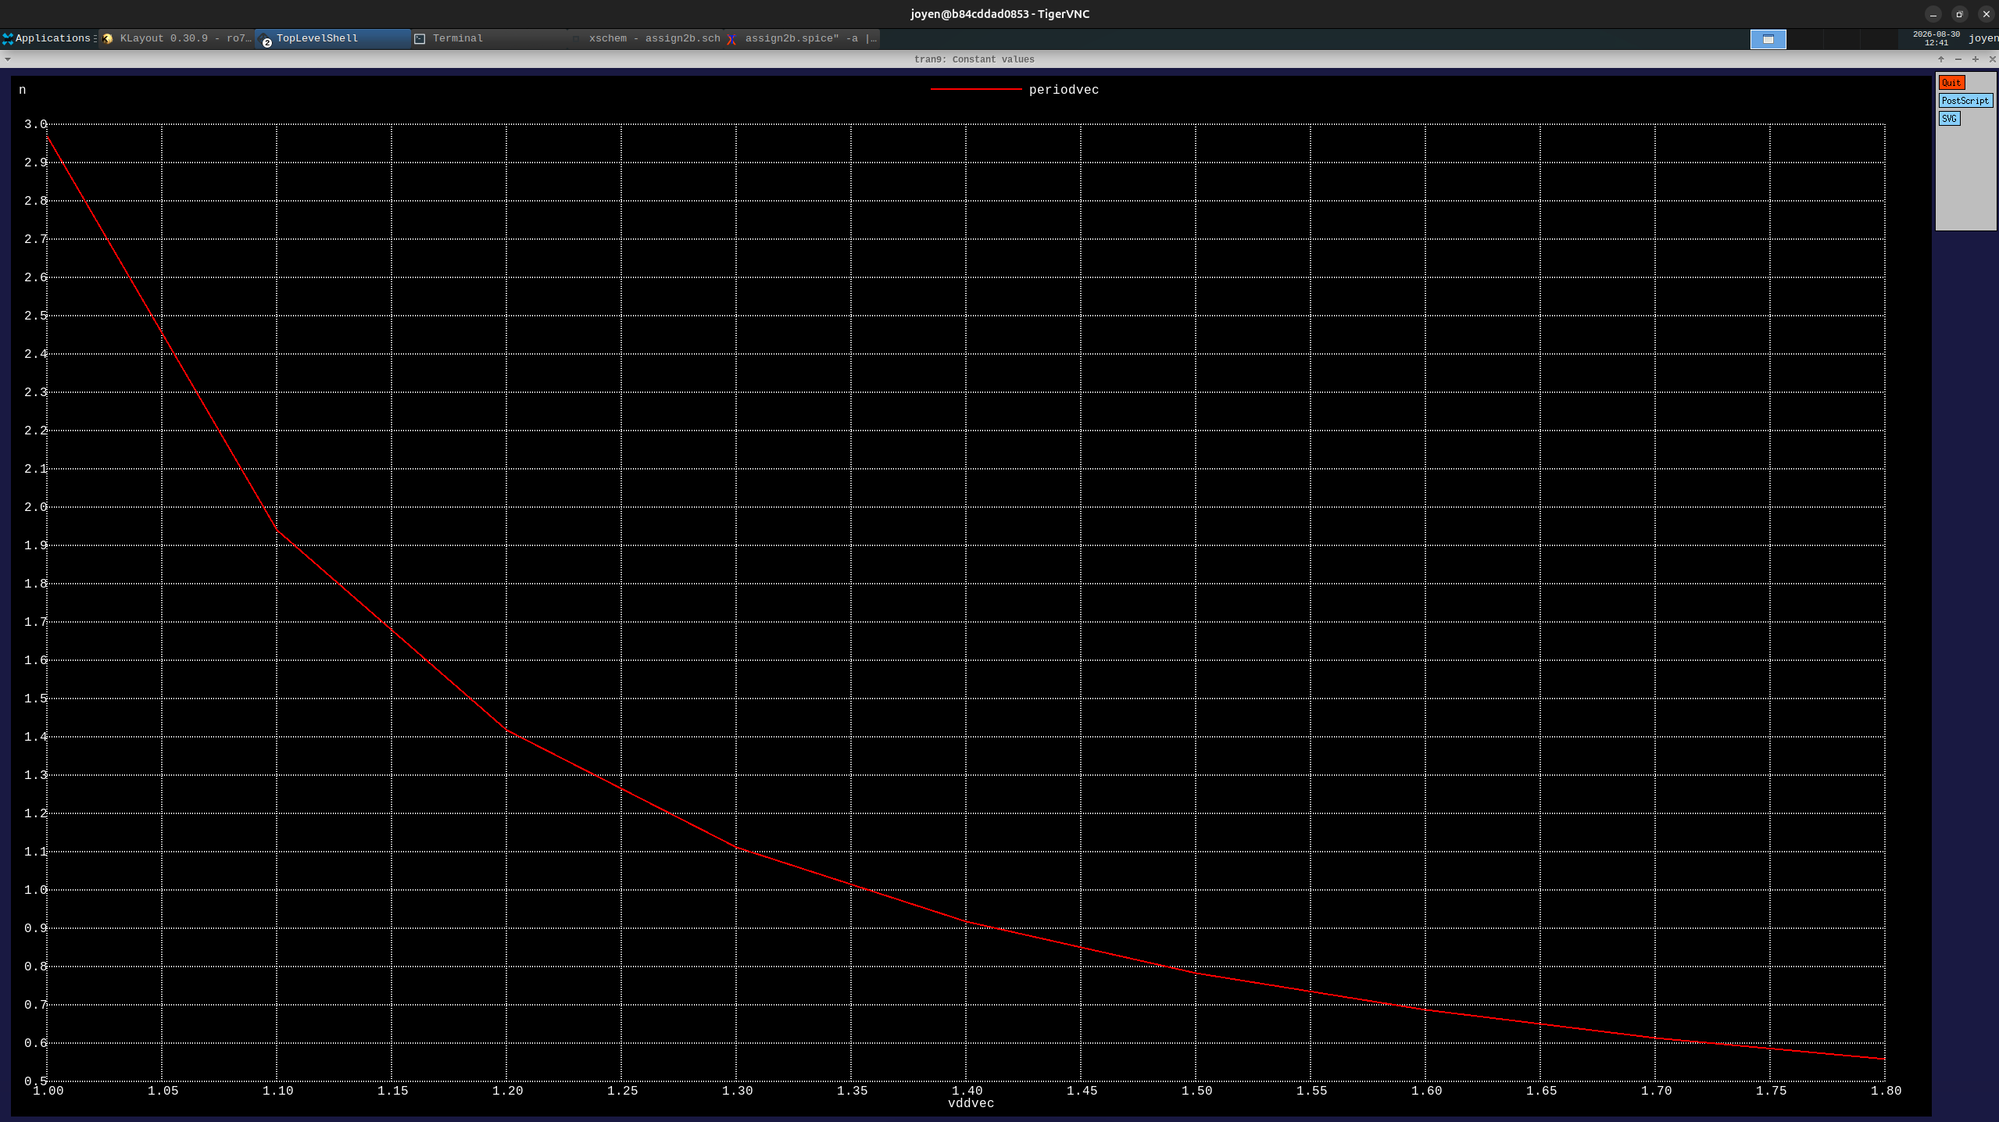
\includegraphics[width=0.9\textwidth]{figures/ro7_period_vs_vdd_2b.png}

\textbf{Figure 9:} period vs $V_{DD}$

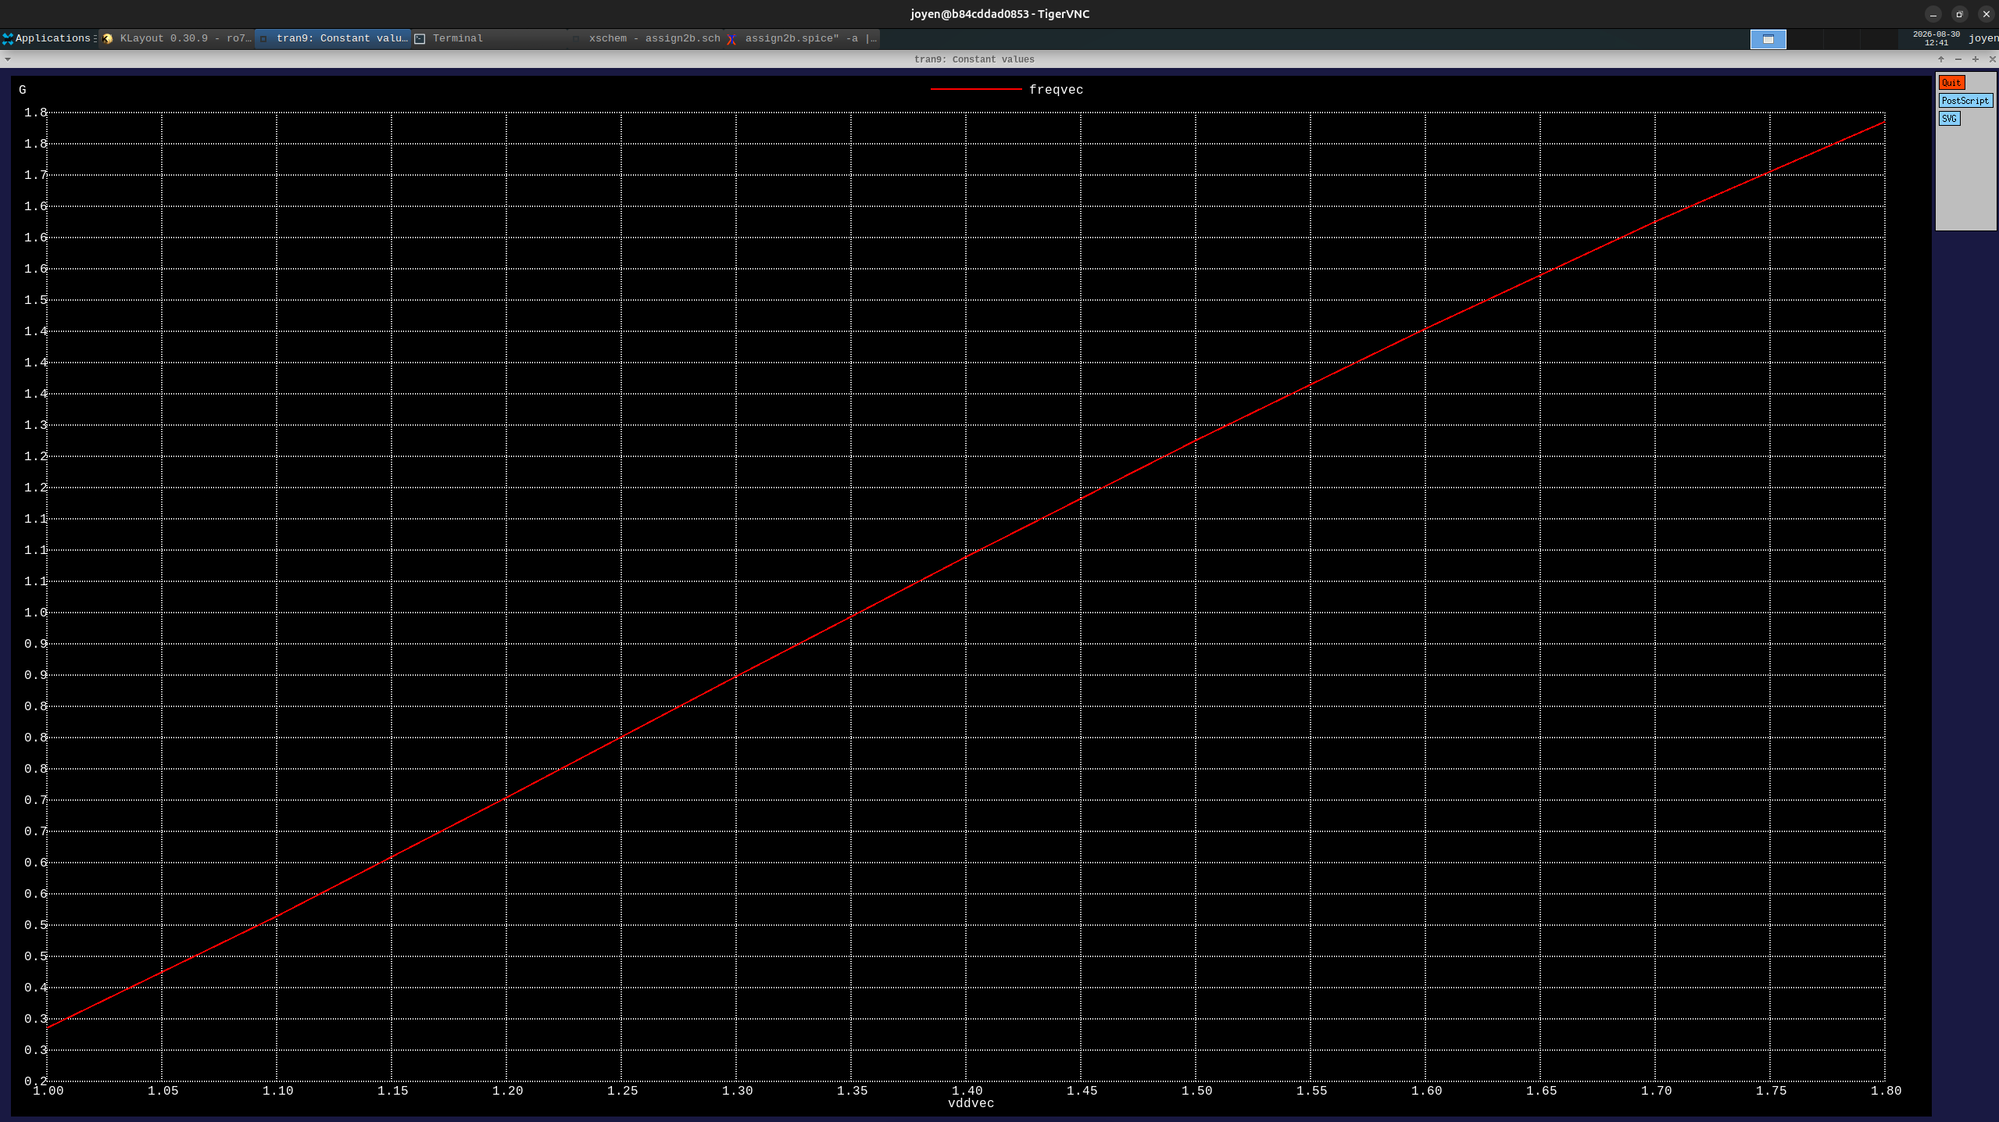
\includegraphics[width=0.9\textwidth]{figures/ro7_freq_vs_vdd_2b.png}

\textbf{Figure 10:} frequency vs $V_{DD}$

Period decreases monotonically (from $\approx 3$~ns at $V_{DD}=1.0$V down to
$\approx 0.56$~ns at $V_{DD}=1.8$V) and frequency increases correspondingly
(from $\approx 0.33$~GHz to $\approx 1.79$~GHz) as $V_{DD}$ increases from
1.0V to 1.8V.
%%------------------------------------------------------------------------------
\subsection{Compare the frequencies against pre-layout simulation in Assignment 3}

\subsubsection{Schematic}
Same $V_{DD}$-sweep testbench as Section~2.2.1 (\texttt{assign2b.sch}, this
assignment) vs.\ the schematic-only (no layout parasitics) 7-stage ring
oscillator testbench from Assignment 3, Part 2(b).

\subsubsection{Layout}
Same ring oscillator layout as Section~2.1.2 (\texttt{ro7.gds}); Assignment 3
has no layout (schematic-only, pre-extraction).

\subsubsection{Measurement}

\begin{table}[h]
  \centering
  \begin{tabular}{|c|c|c|c|c|}
    \hline
    $V_{DD}$ (V) & Pre-layout $T$ (ns) & Post-layout $T$ (ns) & Pre-layout $f$ (GHz) & Post-layout $f$ (GHz) \\
    \hline
    1.0 & 2.07  & 2.97  & 0.483 & 0.337 \\
    1.1 & 1.71  & 1.95  & 0.585 & 0.513 \\
    1.2 & 1.34  & 1.40  & 0.746 & 0.714 \\
    1.3 & 1.00  & 1.10  & 1.000 & 0.909 \\
    1.4 & 0.80  & 0.90  & 1.250 & 1.111 \\
    1.5 & 0.65  & 0.78  & 1.538 & 1.282 \\
    1.6 & 0.545 & 0.68  & 1.835 & 1.471 \\
    1.7 & 0.465 & 0.605 & 2.151 & 1.653 \\
    1.8 & 0.409 & 0.560 & 2.444 & 1.787 \\
    \hline
  \end{tabular}
  \caption{Pre-layout (Assignment 3, Part 2(b)) vs.\ post-layout (this
  assignment, Section 2.2) 7-stage ring oscillator period/frequency vs.\
  $V_{DD}$. All values read off the respective \texttt{periodvec}/\texttt{freqvec}
  plots, except $V_{DD}=1.8$~V which is the exact \texttt{meas} value in each
  case.}
  \label{tab:2c-compare}
\end{table}

The post-layout ring oscillator is consistently slower than the pre-layout
(schematic-only) simulation across the whole $V_{DD}$ sweep -- e.g.\ at the
calibrated $V_{DD}=1.8$~V point, period increases from $0.409$~ns to
$0.560$~ns ($\approx 37\%$ higher) and frequency drops from $2.444$~GHz to
$1.787$~GHz ($\approx 27\%$ lower). This is expected: the extracted layout
adds parasitic wire resistance and capacitance (\texttt{ro7\_extracted.spice})
on top of the intrinsic device capacitance assumed in the schematic-only
Assignment 3 simulation, slowing every stage down and lowering the achievable
oscillation frequency.
